%%%%%%%%%
%
% Trade 
% Notes of research
% Brian Dew
%
%%%%%%%%%
	\documentclass[10pt,letterpaper]{article}

%
% Packages
%
	\usepackage[right=1.6in, left=1.6in, top=1.3in, bottom=1.2in]{geometry}
	\usepackage{pgfplots,pgfplotstable}
	\usepackage{amsmath,amsthm,amssymb}	
	\usepackage{graphicx}
	\usepackage[colorlinks,
  		linkcolor=cyan!50!blue,
  		filecolor=cyan!50!blue,
 		citecolor=cyan!50!blue,
 		urlcolor=cyan!50!blue,
 		linktoc=all]{hyperref}
	\usepackage{calc}
	\usepackage[latin1]{inputenc}
	\usepackage{float}
	\usepackage{array}
	\usepackage{booktabs}
	\usepackage[center]{caption}
	\usepackage{xcolor}
	\usepackage[eulergreek]{sansmath}
	\usepackage{listings}
	\usepackage{parskip}
	\usepackage{bm}

%
% Title Info
%

	\author{Brian Dew\\ (brian.dew@american.edu)}
	\title{Trade Network Structure and Export Volatility}

\tikzset{
    	every node/.append style={font=\sansmath\sffamily\footnotesize}}

\begin{document}
\maketitle

\section{Theoretical background}
Xavier Gabaix (2011) offered theoretical and empirical evidence against the argument of Lucas (1977) that firm-specific shocks average out. Gabaix showed that 1/3 of output volatility in the United States can be directly tied to changes in the 100 largest U.S. firms. When firm sizes follow a power-law distribution, idiosyncratic shocks do not average out, and actually propagate downstream and affect aggregate economic output. This is because there are often few central suppliers for the key inputs to several industries. A shock to one the central firms causes consequences for all firms that require the input for their own production. I hypothesize that this relationship holds internationally, particularly given actual variation in the volume of exports by product and country, and the rise of international trade of intermediate goods due to global value chains.

\section{Building the argument}
Three basic points to my argument:

\begin{enumerate}
\item Countries need goods to produce goods (Leontief I-O linkages). Inputs from upstream suppliers are required to produce outputs for downstream consumers.
\item Countries role in the trade of individual goods (specifically their \href{https://en.wikipedia.org/wiki/Centrality}{centrality}) is not uniform, and for some goods, follows a power law distribution \footnote{Defined for this paper as having an estimated alpha value of weighted outdegree centrality scores between 2 and 3, where $p(x) = Cx^{-\alpha}$.}. The extent of this distribution varies from product to product, and can be captured for each product by applying the tools of network analysis.
\item Shocks from upstream are propagated downstream depending on the network structure for the affected product. 
\end{enumerate}

Essentially, this is an argument about how network structure affects whether idiosyncratic shocks propagate or die out. Internationally, does the trade network's tendency to have central exporters affect whether a supply-shock to the imports of an intermediate good are passed-through and reduce exports?

The motivation for this research comes from an anomaly noticed following two recent natural disasters. First, the 2011 Tohoku earthquake and tsunami, which caused massive destruction, loss of life, and a nuclear disaster, also caused supply-shocks in global trade. French automakers were forced to shutter assembly lines after diesel engine imports from Japan were delayed. Likewise, the launch of the iPad 2 was delayed when the Japanese supplier of the cover glass was affected by the disaster. Second, the 2011 Thailand floods disrupted the production of computer hard disk drives, which has been dominated by Thai producers. The price of hard disk drives nearly doubled worldwide and remained elevated for two years. Such disruptions to the supply of key intermediate goods can create a situation where a localized supply-shock (from a natural disaster) results in aggregate fluctuations elsewhere in the world.

\section{Visual representation}
\vspace{1mm}
\begin{figure}[h]
\caption[]{The effect of a negative shock to Australian iron ore exports depends on network structure. Here circles represent countries, with Australia (AUS) as the localized supply-shock affected country, in orange, countries without a functioning supplier in yellow, and unaffected countries in blue\footnotemark. Solid lines represent unaffected trade flows and dashed lines represent compromised trade flows.} \label{fig:M1}
\centering
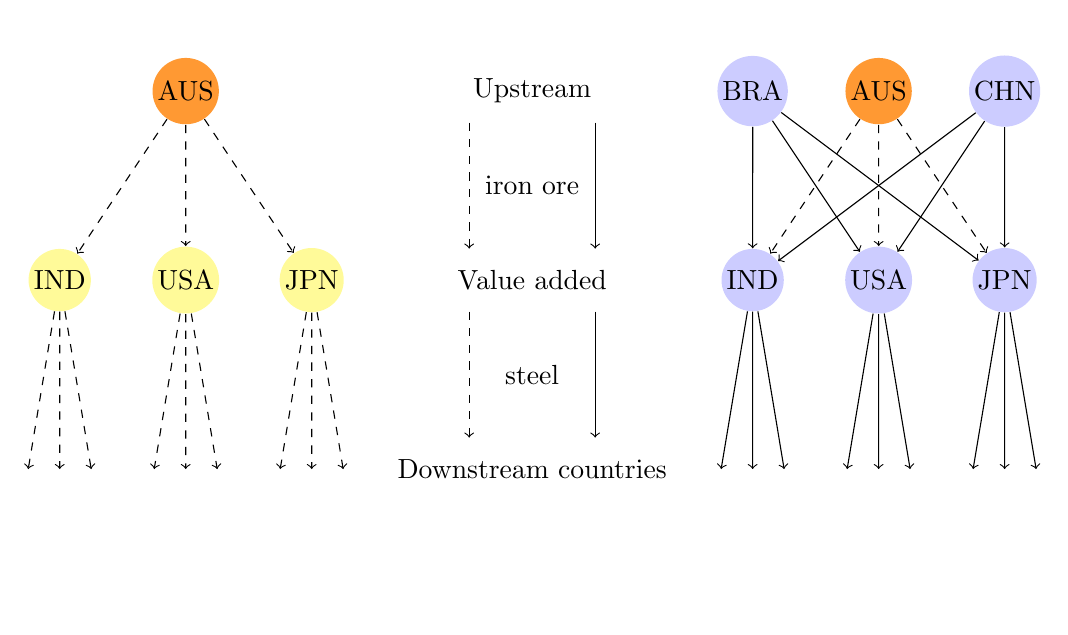
\begin{tikzpicture}
  [scale=.8,auto=left,every node/.style={inner sep=1pt,circle,fill=yellow!40}]
  \node [fill=orange!80] (n6) at (3,10) {AUS};
  \node [draw=none,fill=none] (n7) at (8.5,10) {Upstream};
  \node [draw=none,fill=none] (n8) at (8.5,7) {Value added};
  \node [draw=none,fill=none] (n9) at (8.5,8.5) {iron ore};
  \node [draw=none,fill=none] (n10) at (8.5,4) {Downstream countries};
  \node [draw=none,fill=none] (n11) at (8.5,5.5) {steel};
  \node (n4) at (5,7)  {JPN};
  \node (n5) at (1,7)  {IND};
  \node (n3) at (3,7)  {USA};
  \draw [->, dashed] (7.5,9.5) -- (7.5,7.5);
  \draw [->] (9.5,9.5) -- (9.5,7.5);
  \draw [->, dashed] (7.5,6.5) -- (7.5,4.5);
  \draw [->] (9.5,6.5) -- (9.5,4.5);
  \draw [->, dashed] (n4) -- (5,4);
  \draw [->, dashed] (n4) -- (4.5,4);
  \draw [->, dashed] (n4) -- (5.5,4);
  \draw [->, dashed] (n5) -- (1,4);
  \draw [->, dashed] (n5) -- (0.5,4);
  \draw [->, dashed] (n5) -- (1.5,4);
  \draw [->, dashed] (n3) -- (3,4);
  \draw [->, dashed] (n3) -- (2.5,4);
  \draw [->, dashed] (n3) -- (3.5,4);
  
  \foreach \from/\to in {n6/n4,n6/n5,n6/n3}
    \draw[->, dashed] (\from) -- (\to);
    
  \node [fill=orange!80] (p6) at (14,10) {AUS};
  \node [fill=blue!20] (p2) at (12,10) {BRA};
  \node [fill=blue!20] (p1) at (16,10) {CHN};  
  \node [fill=blue!20] (p4) at (16,7)  {JPN};
  \node [fill=blue!20] (p5) at (12,7)  {IND};
  \node [fill=blue!20] (p3) at (14,7)  {USA};
  \draw [->] (p4) -- (16,4);
  \draw [->] (p4) -- (15.5,4);
  \draw [->] (p4) -- (16.5,4);
  \draw [->] (p5) -- (12,4);
  \draw [->] (p5) -- (11.5,4);
  \draw [->] (p5) -- (12.5,4);
  \draw [->] (p3) -- (14,4);
  \draw [->] (p3) -- (13.5,4);
  \draw [->] (p3) -- (14.5,4);

  \foreach \from/\to in {p2/p3,p2/p4,p2/p5,p1/p5,p1/p3,p1/p4}
    \draw[->] (\from) -- (\to);
    
  \foreach \from/\to in {p6/p4,p6/p5,p6/p3}
 	\draw[->, dashed] (\from) -- (\to);
\end{tikzpicture}
\end{figure}
\footnotetext{There may still be price effects.}
\vspace{-15mm}
\section{Borrowing a model}

The derivation from theory of a testable hypothesis is borrowed almost verbatim from Acemoglu, Akcigit, and Kerr (2016) but adjusted to apply internationally (and to ignore demand shocks) as follows:

We start with a Cobb-Douglas production function for each country:
$$ y_i = e^{z_i}l_i^{\alpha_i^l} \prod_{j=1}^{n} x_{ij}^{a_{ij}}$$

Where $x_{ij}$ is the volume of goods produced by country j and imported to country i, $l_i$ is labor, and $z_i$ is a Hicks-neutral productivity shock. Assume that for each country, $\alpha_i^l >0$, and $a_{ij} \geq 0$ for each pair of countries in the network (if $a_{ij} = 0$, there are no imports to country $i$ from country $j$). Lastly,
$$ \alpha_i^l + \sum_{j=1}^{n} a_{ij} = 1$$

so constant returns to scale are assumed. 

The market clearing condition is:
$$y_i = c_i + \sum_{j=1}^{n} x_{ji}$$

where $c_i$ is domestic consumption and an amount of goods is also exported to each of $n$ countries.

The downward sloping line comes from preferences of a representative household:
$$ u(c_1,c_2,...,c_n,l) = \gamma (l) \prod_{i=1}^{n} c_i^{\beta_i}$$

where $\beta_i$ is distributed between 0 and 1, sums to 1 across all $i$'s, and represents the weight of goods from country $i$ in the representative household's preferences. The disutility of labor is given by the function $\gamma (l)$, which is assumed to be negative.

The household faces the following budget constraint:
$$ \sum_{i=1}^{n} p_ic_i = wl$$

where $w$ is the wage rate, set to 1 for simplicity.

Aggregate profit maximization applied to the Cobb-Douglas production functions determines the individual good trade flows (assuming for simplification that trading costs are CIF and incorporated into $p_j$):
$$ \frac{p_jx_{ij}}{p_iy_i} = a_{ij}$$

Consider therefore an international input-output matrix of $a_{ij}$'s denoted as \textbf{A}:
\begin{equation*}
\text{\textbf{A}} = \begin{bmatrix}
		a_{11} & a_{12} & ... \\
		a_{21} & a_{22} &  \\
		\vdots &  & \ddots 
		\end{bmatrix}
\end{equation*}		

The Leontief inverse of matrix \textbf{A} is defined as:
$$ \mathbf{H} \equiv (\mathbf{I} - \mathbf{A})^{-1} $$

with each entry in matrix \textbf{H} identified as $h_{ij}$.

Acemoglu, Akcigit, and Kerr then propose the following relation for the impact of domestic and foreign shocks on changes to aggregate output:
$$ d \ \text{ln} \ y_i = \underbrace{dz_i}_{\text{own effect}} + \underbrace{\sum_{j=1}^{n} (h_{ij} - \bm{1}_{j=i}) \times dz_j}_{\text{network effect}}$$

where $\bm{1}_{j=i}$ is the indicator function for $j=i$.
\section{Data sources and methods}
The primary data source is the BACI dataset produced by CEPII. BACI provides data on bilateral trade by product at the HS six-digit level of disaggregation. BACI is essentially a cleaned and expanded version of UN Comtrade data. 

Supply-shocks are identified using the EM-DAT database of natural disasters. Such supply shocks are by definition exogenous and location specific. 

Data on total exports, the real effective exchange rate, and import and export prices \footnote{Import and export price indices are used to adjust nominal USD trade flow values to constant prices.} are obtained from the IMF's International Financial Statistics (IFS).


\section{Testable hypothesis and econometric model}

To test the theoretical relationship, I will use a variation on the empirical approach of Acemoglu, Akcigit, and Kerr, which is the analog to the previous equation, and specified as follows:
$$ \Delta \ \text{ln} \ Y_{i,t} = \delta_t + \psi \Delta \ \text{ln} \ Y_{i,t-1} + \beta^{own}Shock_{i,t-1} + \beta^{upstream}Shock_{i,t-1} + \varepsilon_{i,t}$$

where $\delta_t$ is the time fixed effect and $\varepsilon_{i,t}$ is the error term. 

So far, I've only slightly modified the theoretical model of Acemoglu, Akcigit, and Kerr. To make their empirical model fit with my hypothesis and the available data\footnote{HS 6-digit.}, I will need to make additional changes, as follows:

\begin{itemize}
\item First, the dependent variable of interest in my model is the log change in real value of total exports of country $i$. This is a representation of the downstream pass-through of an upstream (and in this case cross-border) supply shock. That is, a supply shock to another country will have various domestic effects on consumption baskets and prices, but this work argues that to get to the heart of the question about whether shocks average out or propagate, we need to look at how the downstream is affected.
\item Next, to capture own (domestic) shocks, I will control for changes to exchange rates and relative prices, as measured by the indexed real effective exchange rate (REER) at time $t-1$. This is a domestic determinant of exports that is not correlated with the measures of network structure that I apply next.
\item Lastly, to test the hypothesis that the distribution of exporter sizes affects whether supply shocks propagate or die out, it is critical to measure the upstream (foreign) shock and isolate different shocks by the network structure through which they arrive. This can be done by decomposing previous period intermediate\footnote{All final consumption goods excluded to isolate products which can have downstream affects} goods imports into four categories, defined as follows:
\end{itemize}



	\begin{table}[h]\centering \caption{Categories of intermediate good imports, goods indexed by $k$ \label{mtab}}
	\begin{tabular}{l | c | c}
	\toprule
	 & central players & no central players \\
	 \midrule
	 shock in time $t$ & $M^{cs}_{i,t-1} = \sum_{k=1}^{n} M^{cs}_{k,i,t-1}$ & $M^{ns}_{i,t-1} = \sum_{k=1}^{n}M^{ns}_{k,i,t-1}$ \\
	 \midrule
	 no shock & $M^{cn}_{i,t-1} = \sum_{k=1}^{n} M^{cn}_{k,i,t-1}$ & $M^{nn}_{i,t-1} = \sum_{k=1}^{n}M^{nn}_{k,i,t-1}$ \\
	 \bottomrule
	\end{tabular}
	\end{table}
	
	\vspace{2mm}
	
where $M$ is the real US dollar value of imports to country $i$ from all other countries. I aim to estimate the following equation:
$$ \Delta \text{ln} X_{i,t} = \delta_{t} + \beta_1 \Delta \text{ln} X_{i,t-1} + \beta_2 \Delta q_{i,t-1} + \beta_3 \text{ln} M^{cs}_{i,t-1} + \beta_4 \text{ln} M^{ns}_{i,t-1} + \beta_5 \text{ln} M^{cn}_{i,t-1} + \varepsilon_{i,t} $$

where $\delta_t$ is again the time fixed effects. The second and third terms attempt to control for domestic shocks. Previous period export growth, $\Delta \text{ln} X_{i,t-1}$,  is unrelated to a next period supply shock, as is the previous period change in real effective exchange rate, $\Delta q_{i,t-1}$. The variable of interest, which I hypothesize affects exports of downstream countries, is the previous period ($t-1$) imports of goods with power law distribution exporter sizes when there has been a shock to the production of that good in period $t$, given by $\text{ln} M^{cs}_{i,t-1}$. To control for the possibility that the supply-shock, regardless of exporter sizes, causes the full adjustment in exports, the non-power-law-distributed imports from supply shock countries are included as $\text{ln} M^{ns}_{i,t-1}$. Lastly, to control for the possibility that exporter size distribution affects exports regardless of supply shocks, imports of goods where the exporter country sizes follow a power law distribution are included as $\text{ln} M^{cn}_{i,t-1}$.

My hypothesis is then:

\begin{align*}
\text{H}_0 &: \beta_3 < \beta_4, \quad \text{where:} \ \beta_3 < 0; \\
\text{H}_a &: \beta_3 \geq \beta_4 
\end{align*}

{
\def\sep{0.5em}
\def\fns{\footnotesize}
\def\onepc{$^{\ast\ast}$} \def\fivepc{$^{\ast}$}
\def\tenpc{$^{\dag}$}
\def\legend{\multicolumn{3}{l}{\footnotesize{Significance levels
:\hspace{1em} $\dag$ : 10\% \hspace{1em}
$\ast$ : 5\% \hspace{1em} $\ast\ast$ : 1\% \normalsize}}}
\begin{table}[htbp]\centering
 \caption{Dependent variable: $\Delta \text{ln} X_{i,t}$}
\begin{tabular}{l r @{} l }\hline\hline 
\multicolumn{1}{c}
{\textbf{Variable}}
 & \textbf{Coefficient} \\& \fns{(Std. Err.)} \\ \hline
L1.x\_ch & -0.249&\onepc \\ & \fns{(0.046)} &\\[\sep]
q\_ch & 0.004&\onepc \\ & \fns{(0.001)} &\\[\sep]
cs\_def & 0.037&\onepc \\ & \fns{(0.011)} &\\[\sep]
ns\_def & -0.028&\tenpc \\ & \fns{(0.016)} &\\[\sep]
cn\_def & 0.081&\onepc \\ & \fns{(0.021)} &\\[\sep]
Intercept & -1.007&\fivepc \\ & \fns{(0.393)} &\\[\sep]
\hline
\multicolumn{3}{c}{}\\
\hline N & \multicolumn{2}{c}{560}\\
R$^{2}$ & \multicolumn{2}{c}{0.732}\\
F $ _{(90,469)}$ & \multicolumn{2}{c}{116.174}\\
\hline
\end{tabular}
\end{table}
}

\begin{tabular}{lrrr}
\toprule
          full\_name &        x &  tot\_ch\_x &  $\sigma$ ch\_x \\
                    &          &           &           \\
\midrule
              China &  2343.19 &      0.93 &      0.23 \\
      United States &  1623.41 &      0.48 &      0.17 \\
            Germany &  1492.54 &      0.13 &      0.20 \\
              Japan &   690.20 &     -0.03 &      0.22 \\
             France &   568.34 &      0.14 &      0.20 \\
              Italy &   528.08 &      0.26 &      0.23 \\
        Netherlands &   574.26 &      0.22 &      0.26 \\
     United Kingdom &   481.89 &      0.16 &      0.23 \\
            Belgium &   473.63 &      0.21 &      0.24 \\
 Russian Federation &   497.76 &      0.36 &      0.38 \\
             Canada &   469.94 &      0.21 &      0.31 \\
             Mexico &   397.66 &      0.57 &      0.29 \\
          Singapore &   405.31 &      0.38 &      0.25 \\
       Saudi Arabia &   342.30 &      0.74 &      0.66 \\
              Spain &   323.85 &      0.25 &      0.23 \\
           Malaysia &   233.93 &      0.56 &      0.25 \\
          Australia &   241.24 &      0.80 &      0.41 \\
        Switzerland &   227.61 &      0.32 &      0.21 \\
             Brazil &   225.10 &      0.46 &      0.38 \\
             Poland &   218.89 &      0.47 &      0.24 \\
\bottomrule
\end{tabular}



{
\def\onepc{$^{\ast\ast}$} \def\fivepc{$^{\ast}$}
\def\tenpc{$^{\dag}$}
\def\legend{\multicolumn{4}{l}{\footnotesize{Significance levels
:\hspace{1em} $\dag$ : 10\% \hspace{1em}
$\ast$ : 5\% \hspace{1em} $\ast\ast$ : 1\% \normalsize}}}
\begin{table}[htbp]\centering
 \caption{Estimation results : xtabond
\label{tabresult xtabond}}
\begin{tabular}{l r @{} l c }\hline\hline 
\multicolumn{1}{c}
{\textbf{Variable}}
 & \multicolumn{2}{c}{\textbf{Coefficient}}  & \textbf{(Std. Err.)} \\ \hline
L.x\_ch  &  -0.251&\onepc  & (0.028)\\
q\_ch  &  0.270&  & (0.166)\\
ecx  &  1.914&\onepc  & (0.668)\\
p\_ch  &  0.430&\onepc  & (0.040)\\
Intercept  &  -0.108&\onepc  & (0.032)\\
\hline
\legend
\end{tabular}
\end{table}
}


{
\def\onepc{$^{\ast\ast}$} \def\fivepc{$^{\ast}$}
\def\tenpc{$^{\dag}$}
\def\legend{\multicolumn{4}{l}{\footnotesize{Significance levels
:\hspace{1em} $\dag$ : 10\% \hspace{1em}
$\ast$ : 5\% \hspace{1em} $\ast\ast$ : 1\% \normalsize}}}
\begin{table}[htbp]\centering
 \caption{Estimation results : xtabond
\label{tabresult xtabond}}
\begin{tabular}{l r @{} l c }\hline\hline 
\multicolumn{1}{c}
{\textbf{Variable}}
 & \multicolumn{2}{c}{\textbf{Coefficient}}  & \textbf{(Std. Err.)} \\ \hline
L.x\_ch  &  -0.219&\onepc  & (0.029)\\
q\_ch  &  0.262&  & (0.177)\\
c  &  1.973&\onepc  & (0.686)\\
Intercept  &  -0.001&  & (0.001)\\
\hline
\legend
\end{tabular}
\end{table}
}



{
\def\sep{0.5em}
\def\fns{\footnotesize}
\def\onepc{$^{\ast\ast}$} \def\fivepc{$^{\ast}$}
\def\tenpc{$^{\dag}$}
\def\legend{\multicolumn{3}{l}{\footnotesize{Significance levels
:\hspace{1em} $\dag$ : 10\% \hspace{1em}
$\ast$ : 5\% \hspace{1em} $\ast\ast$ : 1\% \normalsize}}}
\begin{table}[htbp]\centering
 \caption{Eigenvector centrality of imports}
\begin{tabular}{l r @{} l }\hline\hline 
\multicolumn{1}{c}
{\textbf{Variable}}
 & \textbf{Coefficient} \\& \fns{(Std. Err.)} \\ \hline
L.x\_ch & -0.247&\onepc \\ & \fns{(0.028)} &\\[\sep]
q\_ch & 0.260& \\ & \fns{(0.166)} &\\[\sep]
ecm & 2.072&\onepc \\ & \fns{(0.351)} &\\[\sep]
p\_ch & 0.429&\onepc \\ & \fns{(0.040)} &\\[\sep]
Intercept & -0.116&\onepc \\ & \fns{(0.027)} &\\[\sep]
\hline
\multicolumn{3}{c}{}\\
\hline N & \multicolumn{2}{c}{5841}\\
Log-likelihood & \multicolumn{2}{c}{.}\\
$\chi^{2}_{(4)}$ & \multicolumn{2}{c}{197.602}\\
\hline
\legend
\end{tabular}
\end{table}
}


\newpage
\begin{thebibliography}{9}
\bibitem{acemoglu} 
Daron Acemoglu, Ufuk Akcigit, and William Kerr (2016)
\textsl{Networks and the Macroeconomy: An Empirical Exploration}. 
Chapter in NBER book NBER Macroeconomics Annual 2015, Volume 30, Martin Eichenbaum and Jonathan Parker, editors, 276--335.
 
\bibitem{gabaix} 
Xavier Gabaix (2011) \textsl{The Granular Origins of Aggregate Fluctuations}. Econometrica, 79(3), 733--772.

 
\bibitem{lucas} 
Robert R. Lucas, Jr. (1977) \textsl{Understanding Business Cycles}. 
Carnegie-Rochester Conference Series on Public Policy,
Elsevier 5(1), 7--29.
\end{thebibliography} 
\end{document}